\documentclass[11pt]{beamer}
\usepackage[utf8]{inputenc}
\usetheme{Boadilla}
\setbeamertemplate{navigation symbols}{}
\usepackage{lmodern}
\usepackage[T2A]{fontenc}
\usepackage{cmbright}
\usepackage[russian]{babel}
\usepackage{subcaption}
%\usetheme{Darmstadt}

\usetheme{Boadilla}
\setbeamertemplate{navigation symbols}{}

\usepackage{amsmath}
\usepackage{amsfonts}
\usepackage{bm}
\usepackage{graphicx}
%\usepackage[usenames]{color}
\usepackage{colortbl}
% Использовать полужирное начертание для векторов
\let\vec=\mathbf

\DeclareMathOperator{\mathspan}{span}
\DeclareMathOperator{\mathdim}{dim}
\DeclareMathOperator{\rank}{rank}
\DeclareMathOperator{\diag}{diag}

\newcommand\eqdef{\mathrel{\stackrel{\makebox[0pt]{\mbox{\normalfont\tiny def}}}{=}}}

\begin{document}
	\author{Кононыхин Иван Александрович}

	\title[]{Научная и компьютерная коммуникация в современных условиях}
	\subtitle{<<Обнаружение разладки с помощью метода SSA>>}
	%\logo{}
	\institute[]{
		группа 20.М03-мм\\
		Санкт-Петербургский государственный университет\\
		Прикладная математика и информатика
	}
	\date{\number\year}
	\setbeamercovered{transparent}
	\setbeamertemplate{navigation symbols}{}
	\begin{frame}[plain]
		\maketitle 
	\end{frame}

	\begin{frame}
		\centering
		Введение в теорию
	\end{frame}

	\begin{frame}
		\frametitle{Основные обозначения}
		\begin{block}{Обозначения}
			$F^{(1)} = F_{N_1}^{(1)}$, $F^{(2)} = F_{N_2}^{(2)}$ - временные ряды.
			
			$L: 2 \leq L \leq \min(N_1 - 1, N_2)$ - длина окна.
			
			$ U_l^{(1)}, l = 1, \dotsc, L $ --- собственные векторы траекторной матрицы ряда $ F^{(1)} $
			
			$\mathfrak{L}^{(L, 1)}$ --- линейное пространство, натянутое на $L$---сдвинутые векторы ряда $F^{(1)}$, $ d \eqdef dim \; \mathfrak{L}^{(L, 1)} $
			
			$ I = \{i_1, \dotsc, i_r\} $ --- подмножество $ \{1, \dotsc, L\} $
			
			$ \mathfrak{L}_r^{(1)} \eqdef span(U_l^{(1)}, l \in I) $
			
			$ X_1^{(2)}, \dotsc, X_{K_2}^{(2)} $ --- $L$-сдвинутые векторы ряда $F^{(2)} $
		\end{block}
	\end{frame}

	\begin{frame}
		\frametitle{Индекс неоднородности}	
		\begin{block}{Определение}  \textit{Индекс неоднородности}:
			$$ g(F^{(1)}; F^{(2)}) = \frac{\sum\limits_{l=1}^{K_2}\mathrm{dist}^2(X_l^{(2)}, \mathfrak{L}_r^{(1)})}{\sum\limits_{l=1}^{K_2}\|X_l^{(2)}\|^2} = \frac{\sum\limits_{l=1}^{K_2}\;(\|X_l^{(2)}\|^2 - \sum\limits_{i=1}^{r}\langle X_l^{(2)}, U_i^{(1)}\rangle^2)}{\sum\limits_{l=1}^{K_2}\|X_l^{(2)}\|^2} = $$
			$$ = 1 - \frac{\sum\limits_{l=1}^{K_2}\;\sum\limits_{i=1}^{r}\langle X_l^{(2)}, U_i^{(1)}\rangle^2}{\sum\limits_{l=1}^{K_2}\|X_l^{(2)}\|^2}. $$
		\end{block}
		Индекс неоднородности характеризует несоответствие между рядом $F^{(2)}$ и структурой ряда $F^{(1)}$ (описываемого подпространством $ \mathfrak{L}_r^{(1)} $).
		
		$g \in [0, 1]$.
		
	\end{frame}
	\begin{frame}
		\frametitle{Матрица неоднородности}
		\begin{block}{Обозначения}
			$ F_N: F_N = (f_0, \dotsc, f_{N - 1}), N > 2 $ --- исходный временной ряд;
			
			$ F_{i, j} $ --- подряды ряда $ F_N: F_{i, j} = (f_{i}, \dotsc, f_{j}), \; 0 \leq i < j \leq N - 1 $;
			
			$ B $ --- длина базовых подрядов ряда $ F_N: B > L $;
			
			$ T $ --- длина тестовых подрядов ряда $ F_N: T \geq L $;
		\end{block}
		\begin{block}{Определение}
			Матрица $ \mathbf{G} = \mathbf{G}_{B, T} $, состоящая из элементов $g_{ij}$:
			$$g_{ij} = g(F_{i, i+B-1};\;F_{j, j+T-1}), $$ 
			$$1 \leq i \leq N-B+1,\;\;\;\;\; 1 \leq j \leq N-T+1,$$
			есть \textbf{матрица неоднородности} временного ряда $ F_N $.
			
			\bigskip
			$ F_{i, i+B-1} $ --- Базовый подряд.
			
			$ F_{j, j+T-1} $ --- Тестовый подряд.
		\end{block}
	\end{frame}
	\begin{frame}
		\frametitle{Функции обнаружения неоднородности}
		На основе матрицы неоднородности введем функции неоднородности.
		\begin{block}{Определение}
			Ряд $ D_{T,N}^{(r)} $, элементы которого задаются как 
			$$ d_{n-1}^{(r)} \eqdef g(F_{1, B};\; F_{n-T+1, n}), \;\; T \leq n \leq N. $$
			есть \textbf{строковая функция обнаружения}.
		\end{block}
		Обнаружение структурных изменений по отношению к начальной части ряда $ F_N $.
	\end{frame}
	\begin{frame}
		\frametitle{Функции обнаружения неоднородности}
		\begin{block}{Определение}
			Ряд $ D_{B,N}^{(c)} $, элементы которого задаются как 
			$$ d_{n-1}^{(c)} \eqdef g(F_{n-B+1, n};\; F_{1, T}), \;\; B \leq n \leq N. $$
			есть \textbf{столбцовая функция обнаружения}.
		\end{block}
	\end{frame}
	
	\begin{frame}
		\frametitle{Функции обнаружения неоднородности}
		\begin{block}{Определение}
			Ряд $ D_{T+B,N}^{(d)} $, элементы которого задаются как 
			$$ d_{n-1}^{(d)} \eqdef g(F_{n-T-B+1, n-T+1};\; F_{n-T+1, n}), \;\; T + B \leq n \leq N. $$
			есть \textbf{диагональная функция обнаружения}.
		\end{block}
		Поскольку промежуток между базовым и тестовым интервалами отсутствует, данная функция обнаружения может использоваться для обнаружения резких структурных изменений на фоне медленных.
	\end{frame}

	\begin{frame}
		\frametitle{Функции обнаружения неоднородности}
		\begin{block}{Определение}
			Пусть $ T = B $.
			Ряд $ D_{B,N}^{(s)} $, элементы которого задаются как 
			$$ d_{n-1}^{(s)} \eqdef g(F_{n-B+1, n};\; F_{n-B+1, n}), \;\; B \leq n \leq N. $$
			есть \textbf{симметричная функция обнаружения}.
		\end{block}
	\end{frame}

	\begin{frame}
		\begin{block}{Свойство}
			Любой однородный ряд $ F_N $ порождает нулевую матрицу неоднородности, а наличие ненулевых элементов $ g_{ij} $ в этой матрице свидетельствует о нарушении однородности.
		\end{block}
	\end{frame}

	\begin{frame}
		\frametitle{Типы неоднородности}
		\begin{block}{Определение}
			$ Q $ --- момент возмущения.
			
			$ S \geq 0 $ --- длина переходного интервала.
		\end{block}
		Пусть подряды $ F_{1, Q-1} $ и $ F_{Q+S, N} $ ряда $ F_N $ однородны. Обозначим $ d = \mathrm{rank}_L(F_{1, Q-1}) $, $ d_1 = \mathrm{rank}_L(F_{Q+S, N}) $. Пусть $ L \geq \max(d, d_1) $ и $ L \leq Q-1 $ и $ L \leq N-Q-S+1 $. Если $ \mathfrak{L}^{(L)}(F_{1, Q-1}) = \mathfrak{L}^{(L)}(F_{Q+S, N})$ тогда обе однородные части временного ряда соответствуют одному минимальному $ \mathrm{LRR} $ --- случай \textbf{временной} неоднородности. Отсюда вытекает случай \textbf{постоянной} неоднородности.
	\end{frame}

	\begin{frame}
		\frametitle{Вид матрицы неоднородности}
		Пусть $ \max(B, T) < Q $. Предположим, что $ I = \{1, \dots, r\} $ и $ r = d \leq \min(L, B-L+1) $. Тогда все элементы $ g_{ij} $ матрицы $ \mathbf{G}_{B, T} $ равны нулю для $ i+B \leq Q $ и $ j+T \leq Q $. Значения остальных элементов матрицы неоднородности зависят от типа неоднородности и значений параметров.
		
		\begin{figure}[b]
			\centering
			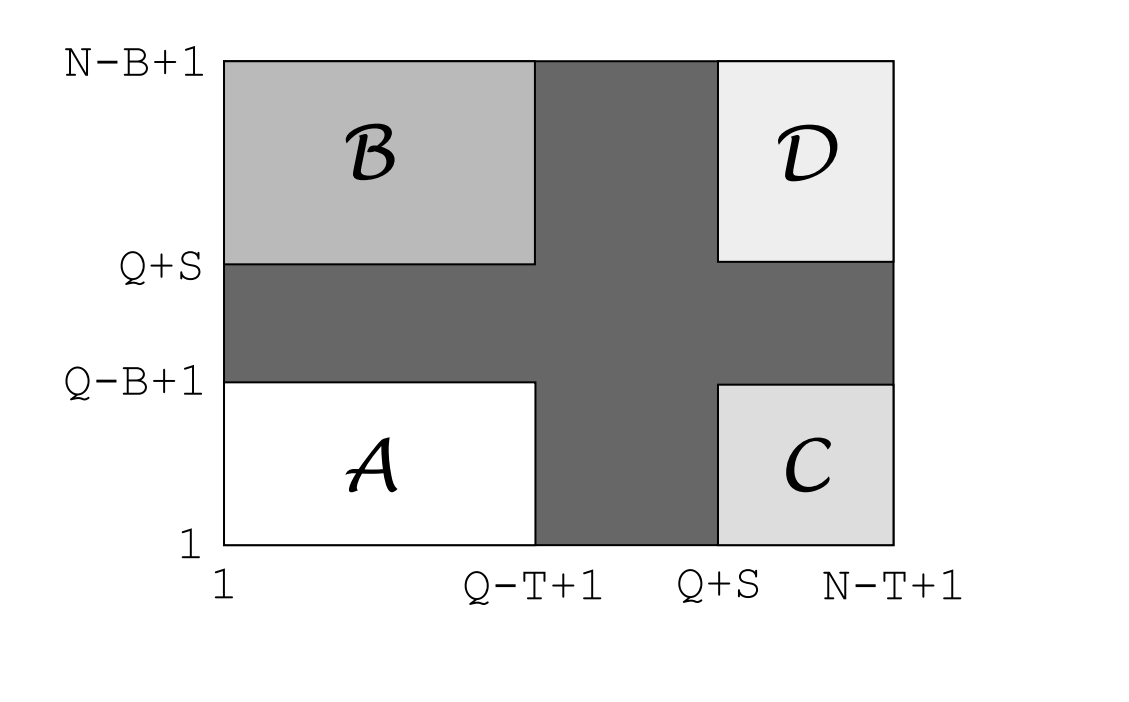
\includegraphics[width=0.7\linewidth]{imgs/H-matrix}
		\end{figure}
	\end{frame}

	\begin{frame}
		\centering
		Сравнение функций обнаружения разладки
	\end{frame}

	\begin{frame}
		\frametitle{Постановка задачи}
		\begin{block}{Задача}
			Эмпирическим путем попытаться оценить, какая из четырех функций обнаружения неоднородности лучше обнаруживает разладку во временном ряде с шумом.
		\end{block}
		
	\end{frame}	
	
	\begin{frame}
		\frametitle{Подготовка эксперимента}
		Рассмотрим ряд $$f_n = 
		\begin{cases}
			C_1\sin(2\pi\omega_1n + \phi_1) + \epsilon, & n < Q, \\
			C_2\sin(2\pi\omega_2n + \phi_2) + \epsilon, & n \geq Q,
		\end{cases}$$
		чьи параметры буду задаваться типом разладки и соответствующим изменением параметров.
		Рассмотрим два типа неоднородности:
		\begin{enumerate}
			\item
			Временную, заданную
			\begin{enumerate}
				\item 
				Фазовым сдвигом: $\phi_1 \neq \phi_2$;
				\item 
				Выбросом:
				$$f_n = 
				\begin{cases}
					C_1\sin(2\pi\omega_1n + \phi_1) & n \neq Q, \\
					10\cdot C_1 & n = Q.
				\end{cases}$$
				\item 
				Изменением амплитуды: $C_1 \neq C_2$.
			\end{enumerate}
			
			\item
			Постоянную, заданную
			\begin{enumerate}
				\item 
				Изменением частоты: $\omega_1 \neq \omega_2$.
			\end{enumerate}
			
		\end{enumerate}
		В качестве оценок качества функций неоднородности будем учитывать скорость возрастания значений и момент преодоления $n_{overcome}$ заданного порога $\delta$.
	\end{frame}

	\begin{frame}
		\frametitle{Параметры}
		$ \omega_1 = \frac{1}{10}, \omega_2 = \frac{1}{5} $
		
		$ C_1 = 1, \; C_2 = 2 $
		
		$ \phi_1=0,\; \phi_2=\frac{\pi}{2} $
		
		$ N = 700, L = 50, \;Q = 301, B = T = 100 $
		
		$ r=d=rank(F_N)=2$.
		
		$\epsilon \sim N(0, \sigma^2)$, $\sigma = 0.5$. 
		
		Для ряда с временной разладкой, заданной изменением амплитуды ($C_1 \neq C_2$), зададим дисперсию шума до разладки как $\frac{\sigma^2}{2}$, чтобы шум $\epsilon$ был пропорционален амплитуде ряда.
		
		\bigskip
		В тестах предполагаем, что момент разладки $Q$ известен и для оценки скорости возрастания будем выводить значения функций в точках $[Q, Q+10, Q+20, Q+30]$.
		
		Порог $ \delta $, относительно которого будем определять, какая из функций неоднородности раньше обнаруживает разладку зададим в  соответствии с промоделированными значениями, описанными далее.
		
		
	\end{frame}

	\begin{frame}
		\frametitle{Ряды}
		\begin{figure}[h]
			\center{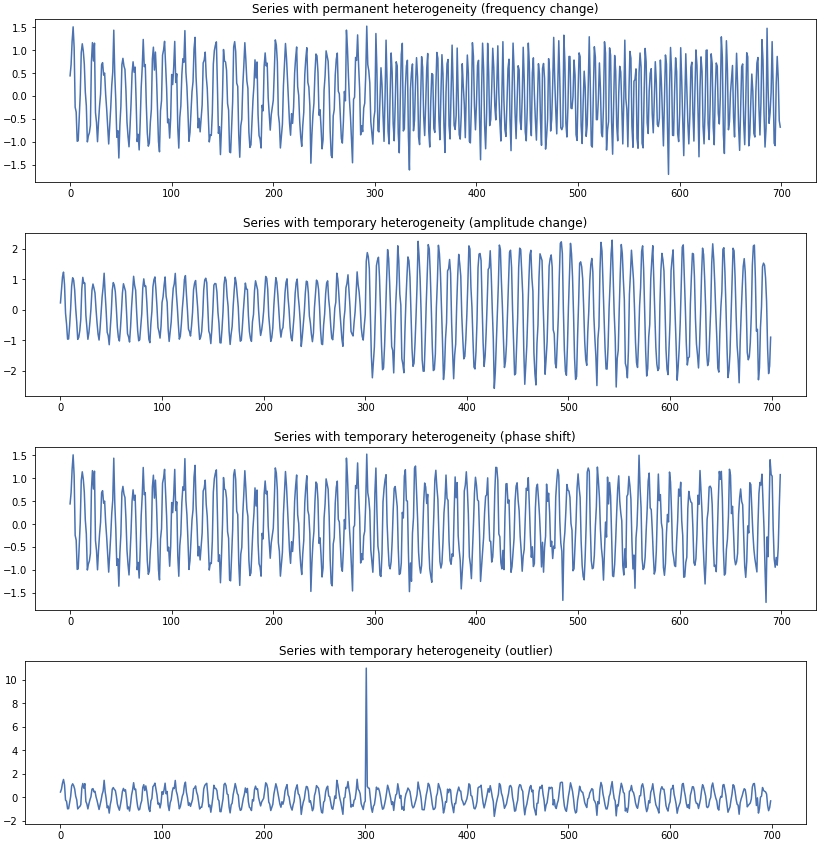
\includegraphics[width=0.65\linewidth]{imgs/seriesNoisedTests}}
		\end{figure}
	
	\end{frame}

	\begin{frame}
		\frametitle{Матрицы неоднородности взятых рядов}
		\begin{figure}[b]
			\centering
			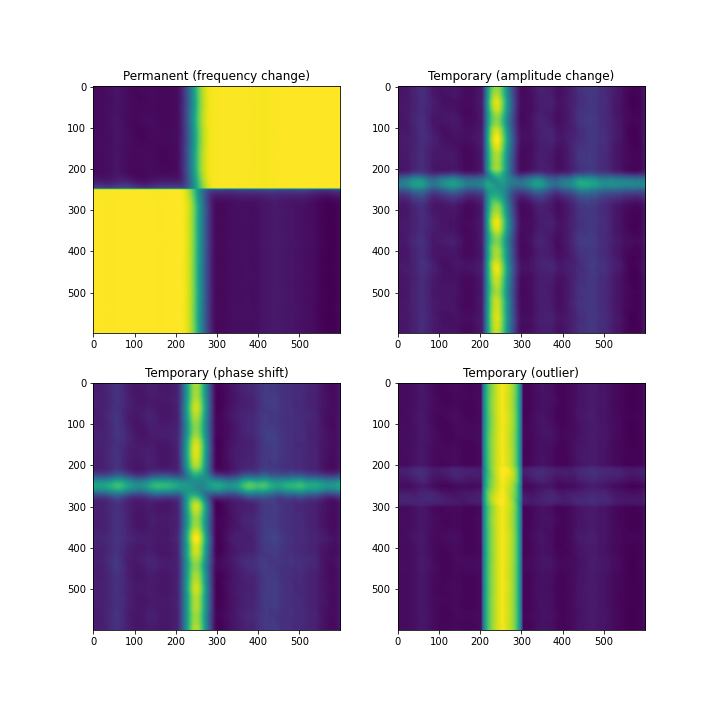
\includegraphics[width=0.75\linewidth]{imgs/heterogeneity_types_noised}
		\end{figure}
		
	\end{frame}

	\begin{frame}
		\frametitle{Функции неоднородности взятых рядов}
		\begin{figure}[b]
			\centering
			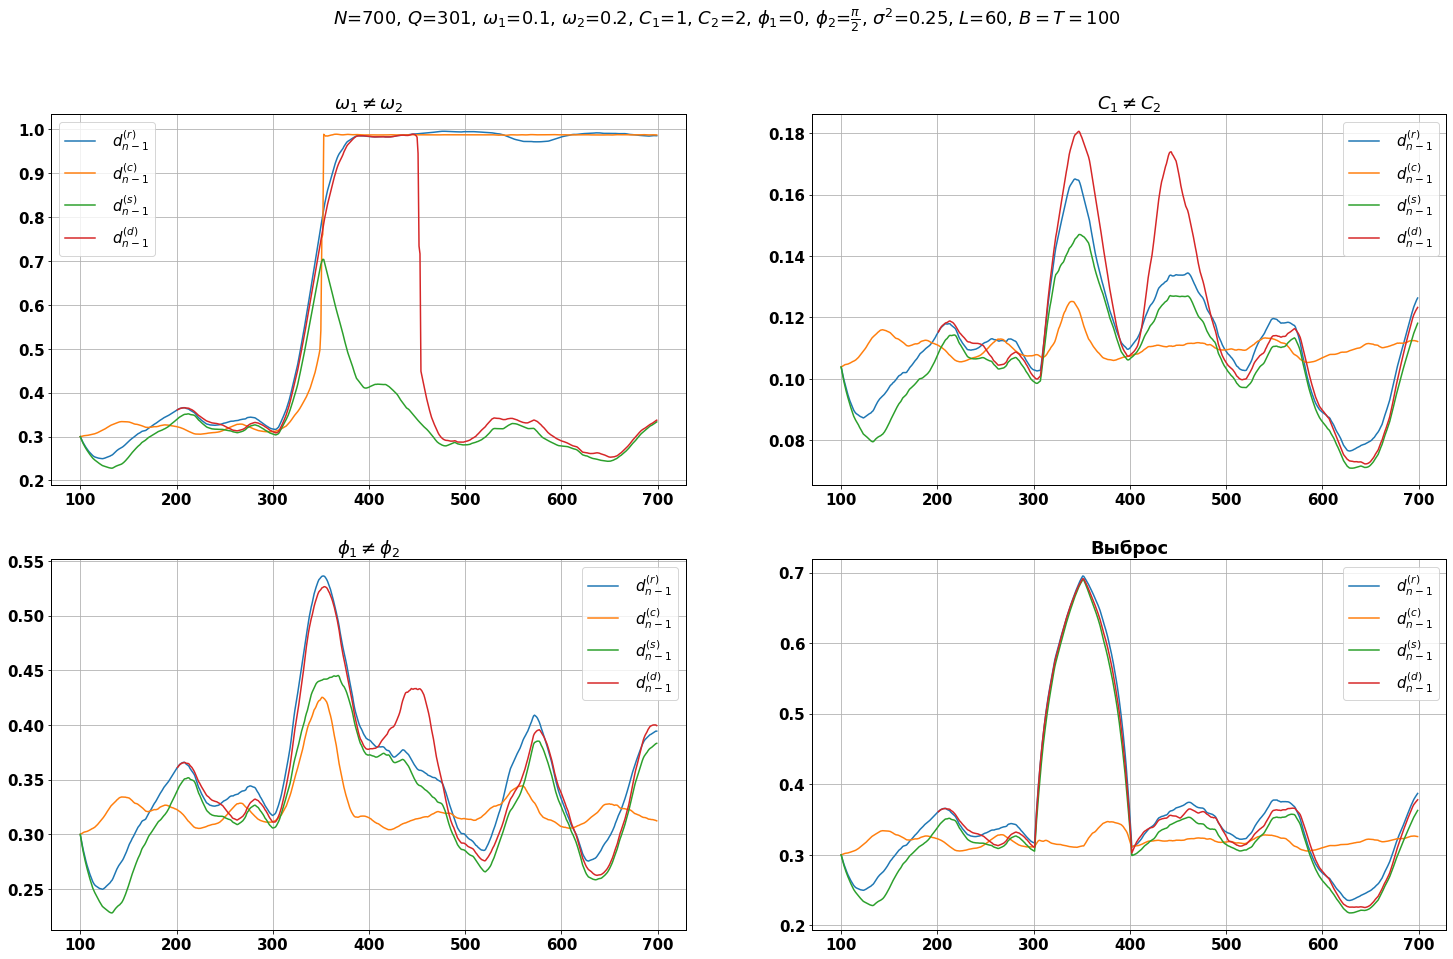
\includegraphics[width=0.65\linewidth]{imgs/detectionNoisedTests}
		\end{figure}
		
	\end{frame}

	\begin{frame}
		\frametitle{Моделирование порога $ \delta $}
		Промоделируем реализации шума $n_{mod}=200$ раз и посчитаем такие характеристики ряда на промежутке $[0, \dots, Q-1]$, как средний максимум и $95$-й процентиль. Эти два значения возьмем в качестве параметра $\delta$. 
		\scriptsize
		\begin{table}[!hhh]
			\caption{Промоделированные пороги $ \delta $}
			\begin{tabular}{llllll}
				Type & Statistic & Row & Col & Sym & Diag \\
				Permanent & Mean max & 0.133 & 0.111 & 0.131 & 0.126  \\
				Permanent & Mean 95 proc & 0.131 & 0.111 & 0.128 & 0.124 \\
				&&&&&\\
				Temporary & Mean max & 0.036 & 0.030 & 0.035 & 0.035  \\
				Temporary & Mean 95 proc & 0.035 & 0.030 & 0.035 & 0.034  \\
				&&&&&\\
				Shifted & Mean max & 0.132 & 0.115 & 0.130 & 0.125  \\
				Shifted & Mean 95 proc & 0.130 & 0.114 & 0.127 & 0.124  \\
				&&&&&\\
				Outlier & Mean max & 0.132 & 0.110 & 0.130 & 0.127  \\
				Outlier & Mean 95 proc & 0.130 & 0.110 & 0.127 & 0.126  \\
			\end{tabular}
		\end{table}
		
	\end{frame}
	
	\begin{frame}
		\frametitle{Результаты оценки для рядов}
		\tiny
		\begin{table}[!hhh]
			\caption{Характеристики функций неоднородности для постоянной разладки ($\omega_1 \neq \omega_2$).}
			\begin{tabular}{llllllll}
				Row & 				   & 		  	  & 			 && Col & 		      & 			      \\
				    & Statistic        & Mean Max 	  & Mean 95 proc && 	& Mean Max     & Mean 95 proc     \\
				    & $\#n_{overcome}$ & 200 	  	  & 200 		 &&     & 200 	      & 200 			  \\
				    & $n_{overcome}$   & 309.12   	  & 308.65      &&     & 313,46       & 313,29 		  \\
				    & Confidence       & $[309.09, 309.15]$& $[308.61, 308.68]$&&     & $[313.35, 313.57]$ & $[313.17, 313.39]$     \\
				    &$f_{n_{overcome}}$& 0.137		  &	0.135		 &&     & 0.1167			  &   0.1165                \\
				Sym & 				   & 		  	  & 			 && Diag& 		      & 			      \\
					& Statistic        & Mean Max 	  & Mean 95 proc && 	& Mean Max     & Mean 95 proc     \\
					& $\#n_{overcome}$ & 200 	  	  & 200 		 &&     & 200 	      & 200 			  \\
					& $n_{overcome}$   & 309.46   	  & 308.94      &&     & 307.78      & 307.45 		  \\
					& Confidence       & $[309.42, 309.49]$ & $[308.91, 308.98]$ &&     & $[307.74, 307.81]$ & $[307.41, 307.48]$     \\
					&$f_{n_{overcome}}$& 0.134		  &	0.131		 &&     & 0.13		 &0,128                   \\
			\end{tabular}
		\end{table}
		\begin{table}[!hhh]
			\begin{tabular}{llllll}
				&              & Row 	  & Col 	& Sym    & Diag  \\
				& $D_Q$        & 0,1085	  & 0,1075 	& 0,1055 & 0,1084		\\
				& $D_{Q+10}$   & 0,1469   & 0,1102  & 0,1416 & 0,1466	\\
				& $D_{Q+20}$   & 0,2405   & 0,1206  & 0,2273 & 0,2400	\\
				& $D_{Q+30}$   & 0,3734	  &	0,1433	& 0,3476 & 0,3727	
			\end{tabular}
		\end{table}
	\end{frame}

	\begin{frame}
		\frametitle{Результаты оценки для рядов}
		\tiny
		\begin{table}[!hhh]
			\caption{Характеристики функций неоднородности для постоянной разладки ($ C_1 \neq C_2 $).}
			\begin{tabular}{llllllll}
				Row & 				   & 		  	  & 			 && Col & 		      & 			      \\
				& Statistic        & Mean Max 	  & Mean 95 proc && 	& Mean Max     & Mean 95 proc     \\
				& $\#n_{overcome}$ & 200 	  	  & 200 		 &&     & 200 	      & 200 			  \\
				& $n_{overcome}$   & 306,885   	  & 306,525      &&     & 306,57       & 306,465 		  \\
				& Confidence       & $[306.86, 306.91]$& $[306.50, 306.55]$&&     & $[306.51, 306.63]$ & $[306.41, 306.52]$     \\
				&$f_{n_{overcome}}$& 0,0373		  &	0,0366		 &&     & 0,0321  &   0,032          \\
				Sym & 				   & 		  	  & 			 && Diag& 		      & 			      \\
				& Statistic        & Mean Max 	  & Mean 95 proc && 	& Mean Max     & Mean 95 proc     \\
				& $\#n_{overcome}$ & 200 	  	  & 200 		 &&     & 200 	      & 200 			  \\
				& $n_{overcome}$   & 307,53   	  & 307,07      &&     & 305,94      & 305,745 		  \\
				& Confidence       & $[307.50, 307.56]$ & $[307.04, 307.10]$ &&     & $[305.91, 305.97]$ & $[305.72, 305.77]$     \\
				&$f_{n_{overcome}}$& 0,0363		  &	0,0357		 &&     & 0,0357		 &0,0354          \\
			\end{tabular}
		\end{table}
		\begin{table}[!hhh]
			\begin{tabular}{llllll}
				&              & Row 	  & Col 	& Sym    & Diag  \\
				& $D_Q$        & 0,0296	  & 0,0297 	& 0,0289 & 0,0296		\\
				& $D_{Q+10}$   & 0,0458   & 0,0331  & 0,0418 & 0,0458	\\
				& $D_{Q+20}$   & 0,0713   & 0,0475  & 0,0537 & 0,0713	\\
				& $D_{Q+30}$   & 0,0876	  &	0,0645	& 0,0536 & 0,0873	
			\end{tabular}
		\end{table}
	\end{frame}

	\begin{frame}
		\frametitle{Результаты оценки для рядов}
		\tiny
		\begin{table}[!hhh]
			\caption{Характеристики функций неоднородности для постоянной разладки ($\phi_1 \neq \phi_2$).}
			\begin{tabular}{llllllll}
				Row & 				   & 		  	  & 			 && Col & 		      & 			      \\
				& Statistic        & Mean Max 	  & Mean 95 proc && 	& Mean Max     & Mean 95 proc     \\
				& $\#n_{overcome}$ & 200 	  	  & 200 		 &&     & 200 	      & 200 			  \\
				& $n_{overcome}$   & 309,37   	  & 308,925      &&     & 311,73       & 311,485 		  \\
				& Confidence       & $[309.33, 309.41]$& $[308.89, 308.96]$&&     & $[311.64, 311.82]$ & $[311.40, 311.57]$     \\
				&$f_{n_{overcome}}$& 0,1351	  &	0,1331		 &&     & 0,1193  &   0,1190         \\
				Sym & 				   & 		  	  & 			 && Diag& 		      & 			      \\
				& Statistic        & Mean Max 	  & Mean 95 proc && 	& Mean Max     & Mean 95 proc     \\
				& $\#n_{overcome}$ & 200 	  	  & 200 		 &&     & 200 	      & 200 			  \\
				& $n_{overcome}$   & 310,105   	  & 309,58      &&     & 307,84      & 307,535 		  \\
				& Confidence       & $[310.06, 310.15]$ & $[309.54, 309.62]$ &&     & $[307.80, 307.88]$ & $[307.50, 307.57]$     \\
				&$f_{n_{overcome}}$& 0,1320		  &	0,1298		 &&     & 0,1282		 &0,1269          \\
			\end{tabular}
		\end{table}
		\begin{table}[!hhh]
			\begin{tabular}{llllll}
				&              & Row 	  & Col 	& Sym    & Diag  \\
				& $D_Q$        & 0,1078	  & 0,1077 	& 0,1050 & 0,1077		\\
				& $D_{Q+10}$   & 0,1421   & 0,1123  & 0,1351 & 0,1421	\\
				& $D_{Q+20}$   & 0,2158   & 0,1347  & 0,1907 & 0,2158	\\
				& $D_{Q+30}$   & 0,3008	  &	0,1836	& 0,2407 & 0,3005	
			\end{tabular}
		\end{table}
	\end{frame}



	\begin{frame}
		\frametitle{Результаты оценки для рядов}
		\tiny
		\begin{table}[!hhh]
			\caption{Характеристики функций неоднородности для постоянной разладки (выброс).}
			\begin{tabular}{llllllll}
				Row & 				   & 		  	  & 			 && Col & 		      & 			      \\
				& Statistic        & Mean Max 	  & Mean 95 proc && 	& Mean Max     & Mean 95 proc     \\
				& $\#n_{overcome}$ & 200 	  	  & 200 		 &&     & 200 	      & 200 			  \\
				& $n_{overcome}$   & 301,935   	  & 301,92      &&     & 303,401       & 303,394		  \\
				& Confidence       & $[301.93, 301.94]$& $[301.916, 301.93]$&&     & $[303.34, 303.46]$ & $[303.33, 303.45]$     \\
				&$f_{n_{overcome}}$& 0,1579	  &	0,1571		 &&     & 0,1185  &   0,1182        \\
				Sym & 				   & 		  	  & 			 && Diag& 		      & 			      \\
				& Statistic        & Mean Max 	  & Mean 95 proc && 	& Mean Max     & Mean 95 proc     \\
				& $\#n_{overcome}$ & 200 	  	  & 200 		 &&     & 200 	      & 200 			  \\
				& $n_{overcome}$   & 301,98   	  & 301,95      &&     & 301,88      & 301,87 		  \\
				& Confidence       & $[301.976, 301.984]$ & $[301.946, 301.953]$ &&     & $[301.876, 301.883]$ & $[301.866, 301.873]$     \\
				&$f_{n_{overcome}}$& 0,1531		  &	0,1517		 &&     & 0,1550		 & 0,1545          \\
			\end{tabular}
		\end{table}
		\begin{table}[!hhh]
			\begin{tabular}{llllll}
				&              & Row 	  & Col 	& Sym    & Diag  \\
				& $D_Q$        & 0,1072	  & 0,1100 	& 0,1042 & 0,1071		\\
				& $D_{Q+10}$   & 0,4369   & 0,1423  & 0,5462 & 0,4366	\\
				& $D_{Q+20}$   & 0,5652   & 0,1459  & 0,1907 & 0,5649	\\
				& $D_{Q+30}$   & 0,6336	  &	0,1387	& 0,6204 & 0,6332	
			\end{tabular}
		\end{table}
	\end{frame}

	\begin{frame}
		\frametitle{Выводы}
		Явными фаворитами являются строковая $d_{n-1}^{(r)}$ и диагональная $d_{n-1}^{(d)}$ функции неоднородности. Они обе показывают превосходство над столбцовой $d_{n-1}^{(c)}$ и симметричной $d_{n-1}^{(s)}$ в устойчивости к шуму $\epsilon$, моментом обнаружения разладки $n_{overcome}$ и скорости возрастания значений $[D_Q, D_{Q+10}, D_{Q+20}, D_{Q+30}]$ после момента нарушения однородности $Q$.
	\end{frame}



	\begin{frame}
		\centering
		Аналитическая оценка индекса неоднородности при изменении частоты гармоники
	\end{frame}

	\begin{frame}
		\frametitle{Постановка задачи}
		\begin{block}{Задача}
			Попробуем аналитически упростить индекс неоднородности $ g $, чтобы явно увидеть, как разности частот ряда до и после разладки влияют на его значения.
		\end{block}
		Рассмотрим ряд
		\begin{equation*} 
			F_N = 
			\begin{cases} 
				C_1\sin(2\pi\omega_1 n + \phi_1),\ n \in [0, Q-1], \\ 
				C_2\sin(2\pi\omega_2 n + \phi_2),\ n \in [Q, N-1]. 
			\end{cases} 
		\end{equation*} 
		Пусть $ \omega_1 \neq \omega_2;\; C_1 = C_2 $. Для простоты зададим амплитуды $ C_1 = C_2 = 1 $.
	\end{frame}


	\begin{frame}
		\frametitle{Индекс неоднородности}
		$$ g(F^{(1)}; F^{(2)}) = \frac{\sum\limits_{l=1}^{K_2}\mathrm{dist}^2(X_l^{(2)}, \mathfrak{L}_r^{(1)})}{\sum\limits_{l=1}^{K_2}\|X_l^{(2)}\|^2} = \frac{\sum\limits_{l=1}^{K_2}\;(\|X_l^{(2)}\|^2 - \sum\limits_{i=1}^{r}\langle X_l^{(2)}, U_i^{(1)}\rangle^2)}{\sum\limits_{l=1}^{K_2}\|X_l^{(2)}\|^2} = $$
		$$ = 1 - \frac{\sum\limits_{l=1}^{K_2}\;\sum\limits_{i=1}^{r}\langle X_l^{(2)}, U_i^{(1)}\rangle^2}{\sum\limits_{l=1}^{K_2}\|X_l^{(2)}\|^2}. $$
	\end{frame}


	\begin{frame}
		\frametitle{Знаменатель}
		$$ \|X_l^{(2)}\|^2 = \sum\limits_{i=1}^{L}(X_{l}^{(2)})_i^2 \approx \int\limits_{0}^{L}\sin^2{(2\pi\omega_2 y + \psi_l)}dy = $$
		$$ = \frac{L}{2} - \frac{\sin(4\pi L\omega_2 + \psi_l) - \sin(2\psi_l)}{8\pi\omega_2} \approx \frac{L}{2}, $$
		при достаточно больших $ L $. 
		
		$ \psi_l $ формируется из $ \phi_2 $ и сдвига, порождаемого номером вектора вложения.
		
		Отсюда $\sum\limits_{l=1}^{K_2}\|X_l^{(2)}\|^2 \approx K_2\cdot\frac{L}{2}$.
	\end{frame}

	\begin{frame}
		\frametitle{Числитель}
		$$ \sum\limits_{l=1}^{K_2}\;\sum\limits_{i=1}^{r}\langle X_l^{(2)}, U_i^{(1)}\rangle^2 = 
		\sum\limits_{l=1}^{K_2}\;\left ( \langle X_l^{(2)}, U_1^{(1)}\rangle^2 + \langle X_l^{(2)}, U_2^{(1)}\rangle^2 \right ) = $$
		$$ =  \sum\limits_{l=1}^{K_2}\; \left [ \left (\sum\limits_{j=1}^{L}(X_{l}^{(2)})_j\cdot (U_{1}^{(1)})_j\right )^2 + \left ( \sum\limits_{j=1}^{L}(X_{l}^{(2)})_j\cdot (U_{2}^{(1)})_j\right )^2 \right ].$$
		
		В силу задания ряда, базисом $ U_{1}^{(1)} $ и $U_{2}^{(1)} $ пространства $ \mathfrak{L}_r^{(1)} $, порожденного элементами $ f_n^{(1)} = \sin(2\pi\omega_1 n + \phi_1) $ являются некие нормированные $ \sin(2\pi\omega_1 n + \psi) $ и $ \cos(2\pi\omega_1 n + \psi) $.
		
		Пусть $ p_1 = \sin(2\pi\omega_1 n + \psi) $, $ p_2 = \cos(2\pi\omega_1 n + \psi) $. Вычислим нормы $ p_1 $ и $ p_2 $ для поиска $ U_{1}^{(1)} $ и $U_{2}^{(1)} $. 
		По аналогии со знаменателем, $ \|p_1\| = \|p_2\| \approx \sqrt{\frac{L}{2}} $, откуда $ U_{1}^{(1)} = \frac{\sin(2\pi\omega_1 n + \psi)}{\sqrt{L/2}} $, $ U_{2}^{(1)} = \frac{\cos(2\pi\omega_1 n + \psi)}{\sqrt{L/2}} $.
		
	\end{frame}

	\begin{frame}
		\frametitle{Числитель}
		Пусть  
		$$ I_l =  \left (\sum\limits_{j=1}^{L}(X_{l}^{(2)})_j\cdot (U_{1}^{(1)})_j\right )^2, $$
		$$ J_l =  \left (\sum\limits_{j=1}^{L}(X_{l}^{(2)})_j\cdot (U_{2}^{(1)})_j\right )^2, $$
		$$ a = \omega_1 + \omega_2,\ b = \omega_1 - \omega_2. $$
	\end{frame}
	\begin{frame}
		\small
		$$ I_l \approx \left( \int\limits_{0}^{L}\sin(2\pi\omega_2 y + \psi_l) \cdot \frac{\sin(2\pi\omega_1 y + \psi)}{\sqrt{L/2}}dy \right)^2 = $$
		$$ = \frac{2}{L} \left(\int\limits_{0}^{L}\sin(2\pi\omega_2 y + \psi_l) \cdot \sin(2\pi\omega_1 y + \psi)dy\right )^2 = $$
		$$ = \frac{2}{L} 
		\left(  
		\frac{\sin(2\pi Lb + \psi - \psi_l) - \sin(\psi - \psi_l)}{4\pi b} - \frac{\sin(2\pi La + \psi + \psi_l) - \sin(\psi + \psi_l)}{4\pi a}
		\right)^2. $$
		
	\end{frame}

	\begin{frame}
		\footnotesize
		$$ J_l \approx \left(\int\limits_{0}^{L}(\sin(2\pi\omega_2 y + \psi_l) \cdot \frac{\cos(2\pi\omega_1 y + \psi)}{\sqrt{L/2}})dy\right)^2 = $$
		$$ = \frac{2}{L}\left(\int\limits_{0}^{L}(\sin(2\pi\omega_2 y + \psi_l) \cdot\cos(2\pi\omega_1 y + \psi))dy\right )^2 = $$
		$$ = \frac{2}{L} 
		\left(  
		\frac{\cos(2\pi Lb + \psi - \psi_l) - \cos(\psi - \psi_l)}{4\pi b} - \frac{\cos(2\pi La + \psi + \psi_l) - \cos(\psi + \psi_l)}{4\pi a}
		\right)^2. $$
		
	\end{frame}

	\begin{frame}
		\begin{block}{Утверждение 1}
			$ \psi = 0 $
		\end{block}
		Т. к. $ \frac{\sum\limits_{l=1}^{K_2}\;\sum\limits_{i=1}^{r}\langle X_l^{(2)}, U_i^{(1)}\rangle^2}{\sum\limits_{l=1}^{K_2}\|X_l^{(2)}\|^2} $ - линейная проекция на пространство $ \mathfrak{L}_r $, эта проекция не должна зависеть от базиса.
		
		\bigskip
		\begin{block}{Предположение 1}
			В сумме по $ l = 1 \dots K_2 $ зависимость от $ \psi_l $ пропадает.
		\end{block}
		Для данного предположения нет теоретически строгого доказательства, однако имперически оно подтверждено.
		
	\end{frame}

	\begin{frame}
		Пусть
		\bigskip
		\small
		$$ I = \left(  \frac{\sin(2\pi Lb)}{4\pi b} - \frac{\sin(2\pi La)}{4\pi a}   \right)^2. $$
		$$ J = \left(  \frac{\cos(2\pi Lb) - 1}{4\pi b} - \frac{\cos(2\pi La) - 1}{4\pi a}  \right)^2. $$
		
		\normalsize 
		Тогда:
		\small
		$$ \sum\limits_{l=1}^{K_2}\;\sum\limits_{i=1}^{r}\langle X_l^{(2)}, U_i^{(1)}\rangle^2 \approx K_2 \cdot \frac{2}{L} \cdot \left [ I + J \right] = $$
		$$ = \frac{K_2 \cdot 2}{L} \cdot \left[ \left(  \frac{\sin(2\pi Lb)}{4\pi b} - \frac{\sin(2\pi La)}{4\pi a}   \right)^2 + \left(  \frac{\cos(2\pi Lb) - 1}{4\pi b} - \frac{\cos(2\pi La) - 1}{4\pi a}  \right)^2 \right] $$
	\end{frame}

	\begin{frame}
		\frametitle{Индекс неоднородности}
		\small
		$$ g(F^{(1)}; F^{(2)}) = 1 - \frac{\sum\limits_{l=0}^{K_2-1}\;\sum\limits_{i=0}^{r-1}\langle X_l^{(2)}, U_i^{(1)}\rangle^2}{\sum\limits_{l=0}^{K_2-1}\|X_l^{(2)}\|^2} \approx $$
		$$ \approx 1 - \frac{\frac{K_2 \cdot 2}{L} \cdot \left[ \left(  \frac{\sin(2\pi Lb)}{4\pi b} - \frac{\sin(2\pi La)}{4\pi a}   \right)^2 + \left(  \frac{\cos(2\pi Lb) - 1}{4\pi b} - \frac{\cos(2\pi La) - 1}{4\pi a}  \right)^2 \right]}{K_2\cdot\frac{L}{2}} = $$
		$$ 1 - \frac{\left[ \left(  \frac{\sin(2\pi Lb)}{4\pi b} - \frac{\sin(2\pi La)}{4\pi a}   \right)^2 + \left(  \frac{\cos(2\pi Lb) - 1}{4\pi b} - \frac{\cos(2\pi La) - 1}{4\pi a}  \right)^2 \right]}{\frac{L^2}{4}}$$
	\end{frame}

	\begin{frame}
		\frametitle{Проверка точности аппроксимации}
		При сравнении индекса неоднородности, вычисленного классическим способом и аналитически упрощенным, результаты оказались довольно похожи, причем при $ L \rightarrow \infty $ оба значения сходятся друг к другу.
		
		\bigskip
		\bigskip
		Зададим параметры:
		
		$ N = 700,\; Q = 301,\; B = 200,\; T = 200 $
		
	\end{frame}

	\begin{frame}
		\frametitle{Проверка точности аппроксимации: изменения $ L $}
		Зафиксируем $ w_1 = \frac{1}{10},\; w_2 = \frac{1}{11} $ и будем изменять $ L $.
		
		\begin{table}[!hhh]
			\centering
			\small
			\begin{tabular}{lll}
				$ L $  & $ g_c $     & $ g_a $       \\
				$ 50 $ & $ 0.518365 $ & $ 0.562352 $ \\
				$ 80 $ & $ 0.890753 $ & $ 0.891823 $ \\
				$ 90 $ & $ 0.955854 $ & $ 0.953909 $
			\end{tabular}
		\end{table}
		
		\begin{figure}[b]
			\centering
			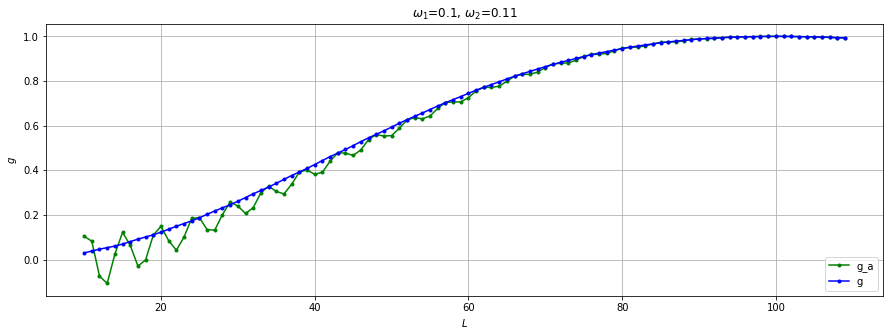
\includegraphics[width=\linewidth]{imgs/dynamics_L}
		\end{figure}
		
	\end{frame}


	\begin{frame}
		\frametitle{Проверка точности аппроксимации: разность $ \omega_1 $ и $ \omega_2 $}
		\begin{block}{Предположение 2}
			Чем сильнее разница $ \omega_1 $ и $ \omega_2 $, тем больше значение $ g $.
		\end{block}
		$ w_1 = \frac{1}{10} $
		
		\begin{figure}[b]
			\centering
			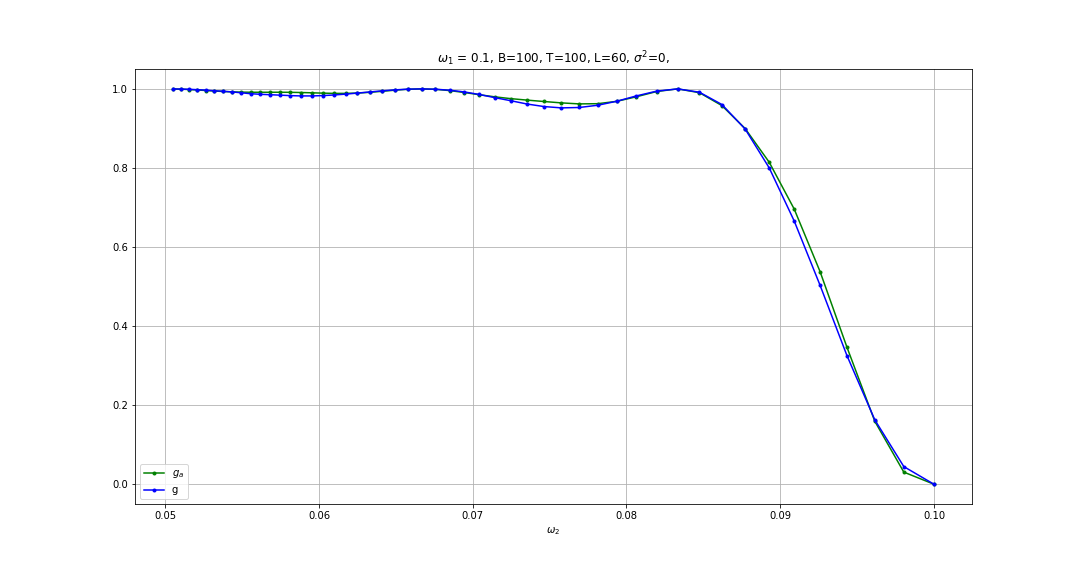
\includegraphics[width=\linewidth]{imgs/dynamics_w2}
		\end{figure}
		
	\end{frame}


	\begin{frame}
		\centering
		Система обнаружения структурной неоднородности ряда с автоматически выстраиваемым порогом срабатывания на основе выведенной аналитической формулы.
	\end{frame}

	\begin{frame}
		\frametitle{Постановка задачи}
		Рассмотрим ряд 
		\begin{equation*} 
			F_N = 
			\begin{cases} 
				C_1\sin(2\pi\omega_1 n + \phi_1),\ n \in [0, Q-1], \\ 
				C_2\sin(2\pi\omega_2 n + \phi_2),\ n \in [Q, N-1]. 
			\end{cases} 
		\end{equation*}
	в котором присутствует разладка в неизвестный момент времени $ Q $. Пусть нам известна начальная частота ряда $ \omega_1 $. Задача системы --- обнаружить разладку при отклонении от начальной частоты ряда $ \omega_1 $ на $ \Delta_{min} $ не позже чем за промежуток времени $ k $. Обозначим $ \omega_{min} = \omega_1 + \Delta_{min} $
	
	\bigskip
	Далее мы будем рассматривать только строковую функцию неоднородности $ d_n^{(r)} $, поэтому обозначим ее как $ d_n $
	\end{frame}

	\begin{frame}
		\frametitle{Предпосылки}
		По теории, чем меньше размер окна $ L $, тем более линеен переходный интервал у $ d_n $. При уменьшении размера окна $ L $ размер векторов вложений также уменьшается, а их количество $ K_2 $ увеличивается, следовательно, при скольжении тестового подряда, начиная с момента $ Q $ векторы вложений ... в сумму числителя индекса неоднородности 
		
		TODO: оставить 10, 30, 60, как на след слайде
		\begin{figure}[b]
			\centering
			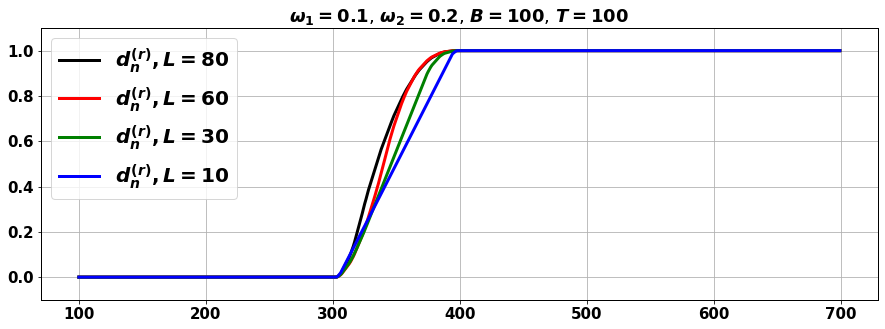
\includegraphics[width=0.8\linewidth]{imgs/row_linear_growth}
		\end{figure}
	\end{frame}

	\begin{frame}
		\frametitle{Предпосылки}
		Благодаря этому наблюдению мы можем аппроксимировать переходный интервал прямой. Длина этого интервала будет равна размеру $ T $ тестовых подрядов. Обозначим эту аппроксимацию как $ a_{T} $.
		
		\begin{figure}[b]
			\centering
			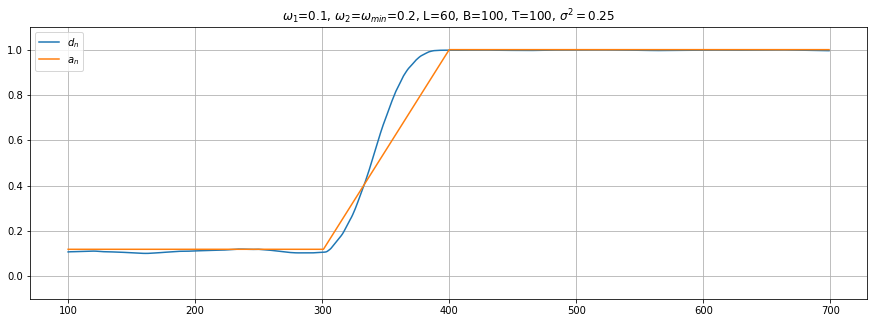
\includegraphics[width=0.65\linewidth]{imgs/row_linear_approximation_1}
		\end{figure}
	
		TODO: Сделать масштаб от 0 до 1
		\begin{figure}[b]
			\centering
			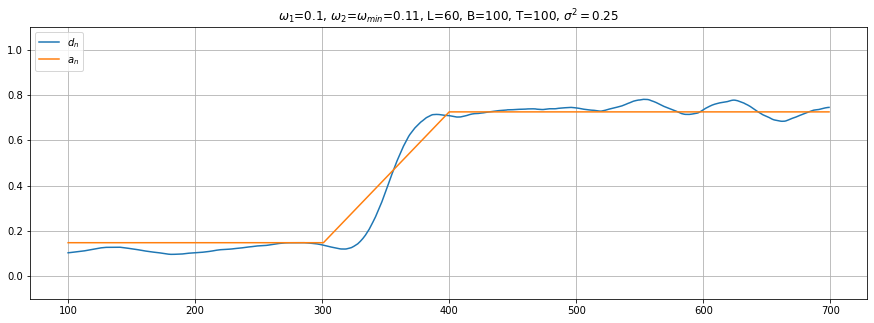
\includegraphics[width=0.65\linewidth]{imgs/row_linear_approximation_2}
		\end{figure}
	\end{frame}

	\begin{frame}
		\frametitle{Реализация}
		Аппроксимируя переходный интервал от $ 0 $ до $ g_a(\omega_1, \omega_{min}) $ прямой, мы получим $ a_T $, имеющая примерный вид переходного интервала функции $ d_{n} $. 

		\bigskip

		Так как по постановке задачи $ \omega_{min} $ --- минимальное изменение частоты для обнаружения неоднородности ряда, то отклонение на $ \Delta \geq \Delta_{min} $ приведут к более высокому значению $ d_n $ после момента $ Q + T $, из-за чего переходный отрезок у $ d_{n} $ будет иметь еще более крутой наклон.
		TODO: 0.2 - \omega_2
		TODO: добавить \omega_2 = 0.3
		\begin{figure}[b]
			\centering
			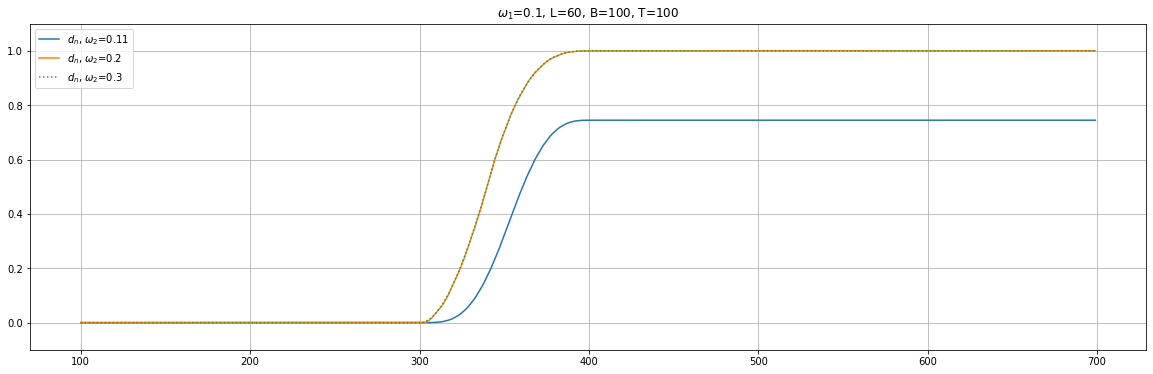
\includegraphics[width=0.9\linewidth]{imgs/diff_omega_growth}
		\end{figure}
		
		
	\end{frame}
	
	\begin{frame}
		\frametitle{Реализация}
		В силу этого, мы можем брать порог $ \gamma $ в точке $ k $ прямой $ a_T $ и сигнализировать об обнаружении неизвестного момента возмущения $ Q $ как момент преодоления этого порога $ \hat{Q} $.
		
		Обозначим это значение как $ \gamma_a $. 
		
		По постановке задачи $ \hat{Q} \in [Q, Q+k] $.
		
		Формализуем систему:
		\begin{itemize}
			\item Входные данные: $\omega_1$, $\Delta_{min}$, $ k $;
			\item Результат: $\hat{Q}$;
			\item Алгоритм:
			\begin{enumerate}
				\item Вычисление $ g_a(\omega_1, \omega_{min}) $;
				\item Аппроксимация переходного интервала $ a_T $;
				\item Фиксирование $ \gamma_a $;
				\item Определение $ \hat{Q} $ как момент преодоления $ d_n $ значения $ \gamma_a $.
			\end{enumerate}	
		\end{itemize}		
		
		
	\end{frame}

	\begin{frame}
		\frametitle{Реализация}
		Зафиксируем параметры: 
		$ \omega_1=\frac{1}{10}, \omega_{min}=\frac{1}{100}, k=30, \omega_2=\frac{1}{5}, Q=301, L=60, B=100, T=100 $.

		\bigskip

	 	При таких параметрах, для графика ниже $ g_a(\omega_1, \omega_{min}) = 0.7252$,  $ \gamma_a = 0.2198$, $ \hat{Q}=326 $.
		\begin{figure}[b]
			\centering
			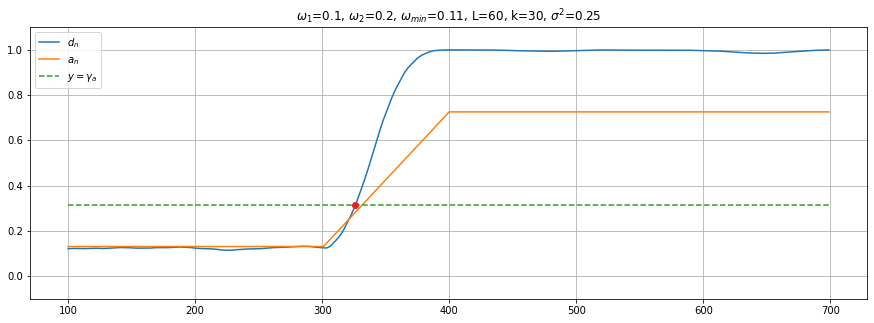
\includegraphics[width=\linewidth]{imgs/example_system_work.png}
		\end{figure}
	\end{frame}
	
	\begin{frame}
		\frametitle{Параметры}
		Все параметры, используемые выше можно разделить на 3 категории: 
		\begin{enumerate}
			\item Заданные формулировкой задачи: $ \omega_1, \omega_{min}, k$;
			\item Неизвестные: $ \omega_2, Q $;
			\item Выбираемые системой: $ L, B, T $.
		\end{enumerate}
		
		Первую категорию параметров можно интерпретировать как заданные пользователем системы. Они фиксированы и не могут меняться для определения более хорошего порога.
		
		\bigskip
		
		Вторая категория зависит от ряда, подаваемого системе и вообще говоря не известны.
		
		\bigskip
		
		Третья категория параметров - те, которые система может подстраивать под тот или иной ряд. Позже попробуем оценить их влияние на оценку системы.
	\end{frame}

	\begin{frame}
		\frametitle{Оценка системы}
		В случае ряда без шума, оценить надежность системы невозможно, так как  $\forall \; \gamma \in [0, \gamma_a] $ покажет стопроцентное определение разладки.
		
		\bigskip
		При добавлении шума, у $ d_{n} $ до момента возмущения появятся колебания и смещается среднее значение. Обозначим дисперсию шума как $ \epsilon_v$.
		
		\begin{figure}[b]
			\centering
			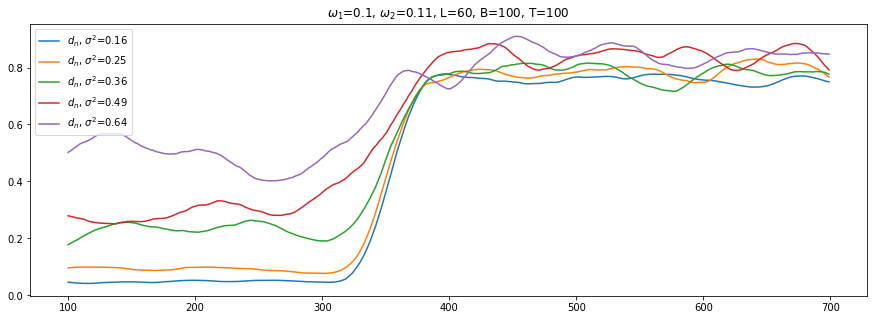
\includegraphics[width=\linewidth]{imgs/row_diff_noise_var}
		\end{figure}
		
	\end{frame}

	\begin{frame}
		\frametitle{Оценка системы}
		Зафиксируем дисперсию шума $ \epsilon_v = 0.25 $ и введем характеристики системы:
		
		\begin{itemize}
			\item $ FPR(\gamma) $ - преодоление порога $ \gamma $ кривой $ d_n $ до момента $ Q $
			\item $ TPR(\gamma) $ - преодоление порога $ \gamma $ кривой $ d_n $ в промежутке $ [Q, Q+k] $
		\end{itemize}
		
		Значения параметров рассмотренных категорий оставим такими же. 
		
		\bigskip
		
		Промоделируем реализации шума $ n_{iter} = 200 $ раз и для $ \forall \gamma \in [0, 1] $ с шагом $ 0.01 $ определим $ FPR(\gamma) $ и $ TPR(\gamma) $.

		Также будем смотреть на $ FPR(\gamma_a) $.
		
	\end{frame}

	\begin{frame}
		\frametitle{Проблема аппроксимации при наличии шума}
		Без шума в ряде, мы знаем, что $ d_{n} $ до момента $ Q $ будет принимать значение $ 0 $, поэтому мы аппроксимируем переходный интервал прямой от $ 0 $ до значения $ \gamma_a $. Однако при наличии шума, значения $ d_{n} $ до разладки смещаются выше, и при задании слишком маленького значения $ \omega_{min} $, система не сможет определить $ \hat{Q} $. 
		
		\begin{figure}[b]
			\centering
			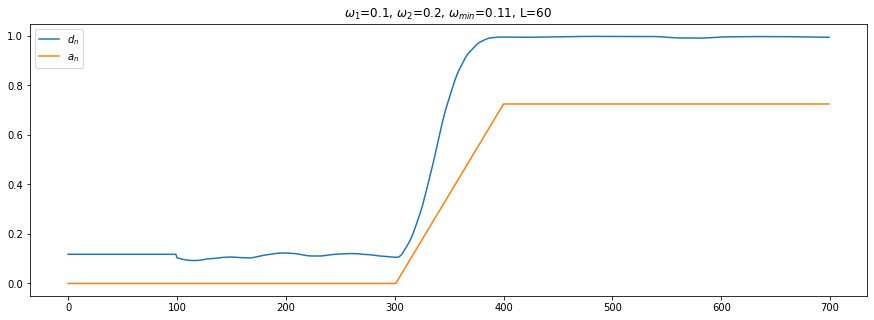
\includegraphics[width=\linewidth]{imgs/noise_existance_problem.png}
		\end{figure}
	\end{frame}

	\begin{frame}
		\frametitle{Проблема аппроксимации при наличии шума}
		В таком случае, нужно ввести предположение о наличии исторических данных без разладки в ряде. На таких данных мы сможем оценить начальное значение $ a_n  $ и аппроксимировать переходный интервал не $ 0 $, а, к примеру, $ 95 $-м процентилем, посчитанном на промежутке, где гарантированно нет неоднородности ряда.
		\begin{figure}[b]
			\centering
			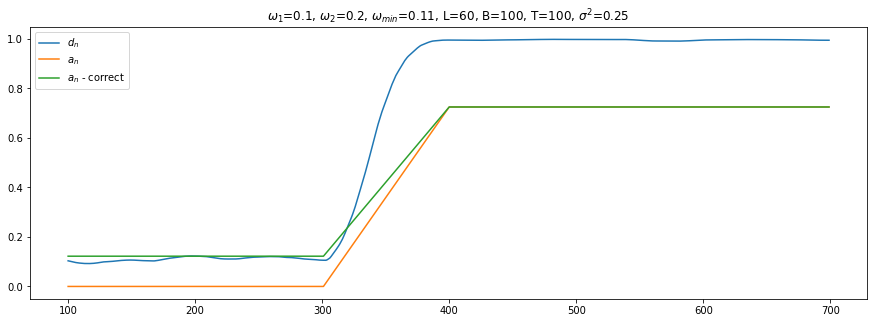
\includegraphics[width=\linewidth]{imgs/noise_existance_problem_solve.png}
		\end{figure}
	\end{frame}


	\begin{frame}
		\frametitle{Оценка системы}
		\begin{figure}[b]
			\centering
			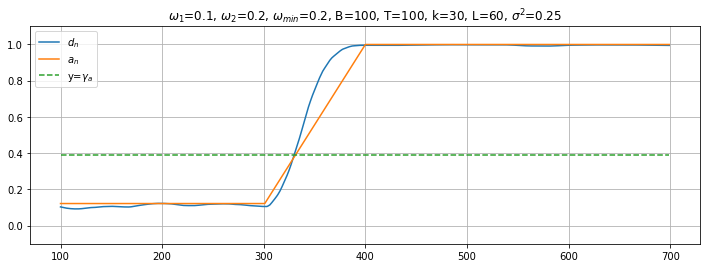
\includegraphics[width=0.85\linewidth]{imgs/system_estimation_one_iter.png}
		\end{figure}
	
		\begin{figure}[b]
			\centering
			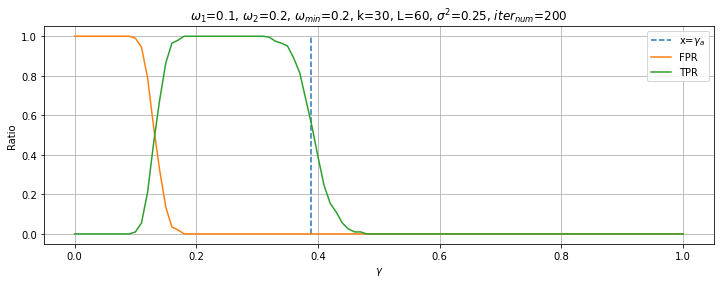
\includegraphics[width=0.85\linewidth]{imgs/system_estimation.png}
		\end{figure}
		
	\end{frame}


	\begin{frame}
		\frametitle{Оценка влияния параметров: T}
		
		\begin{figure}[b]
			\centering
			\subfloat{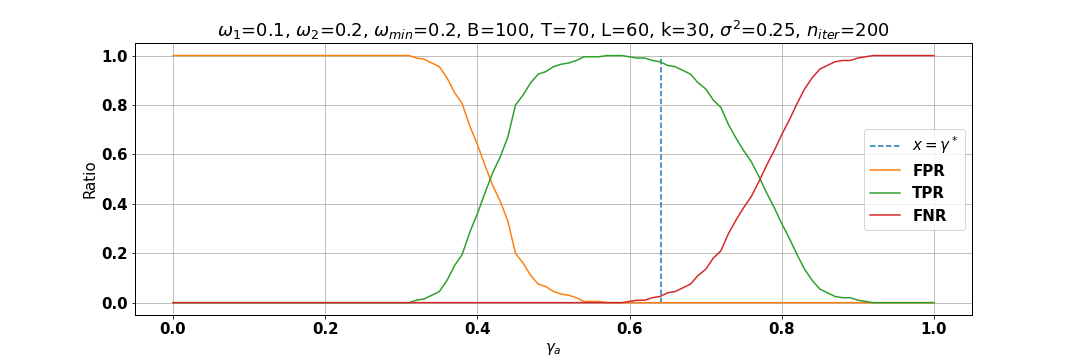
\includegraphics[width=0.7\linewidth]{imgs/system_estimation_T=70.png}}
			
			\smallskip
			\subfloat{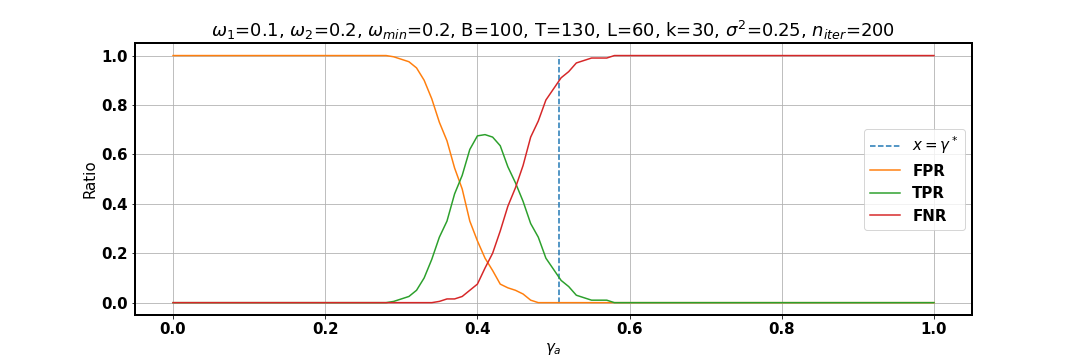
\includegraphics[width=0.7\linewidth]{imgs/system_estimation_T=130.png}}
		\end{figure}
		
		Из изображений видно, что влияя на параметр $ T $ мы можем регулировать устойчивость порога к шуму.
		
	\end{frame}

	\begin{frame}
		\frametitle{Оценка влияния параметров: T}
		Уменьшая $ T $, мы можем сделать $ \gamma_a $ устойчивее к шуму. Однако при $ T \rightarrow L $, количество элементов в тестовых рядах для подсчета индекса неоднородности $ g $ сокращается, усиливая влияние шума на подсчет элементов $ d_{n} $ и приводит к усилению колебаний и увеличению $ FPR(\gamma) $.
		
		\begin{figure}[b]
			\centering
			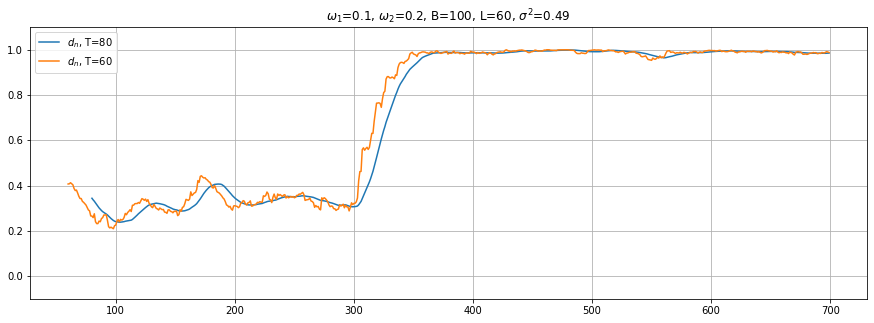
\includegraphics[width=\linewidth]{imgs/decreasing_T.png}
		\end{figure}
	\end{frame}

	\begin{frame}
		\frametitle{Оценка влияния параметров: L}
		Как было отмечено ранее, сходимость $ g_a $ и $ g $ достигается при достаточно больших $ L $. 
		
		\bigskip
		
		Изменяя параметр $ L $, мы регулируем скорость возрастания кривой $ d_{n} $. Таким образом, подстраивая параметр $ L $ мы можем определять $ \hat{Q} $ раньше момента $ Q + k $.
		
		\begin{figure}[b]
			\centering
			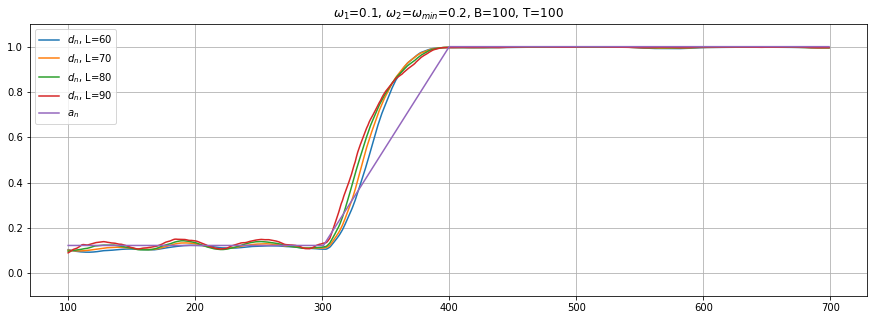
\includegraphics[width=\linewidth]{imgs/row_diff_L.png}
		\end{figure}
		
		
	\end{frame}

	\begin{frame}
		\frametitle{Оценка влияния параметров: B}
		В целом, параметр $ B $ не влияет на устойчивость системы в силу предположении о наличии исторических данных и отсутствия влияния на переходный интервал $ d_n $.
				
		\begin{figure}[b]
			\centering
			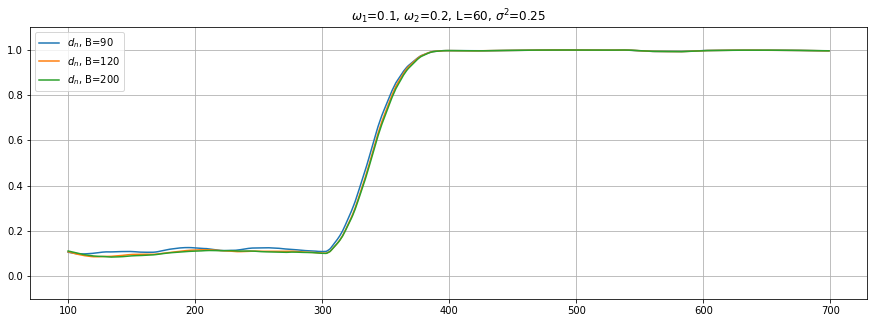
\includegraphics[width=0.85\linewidth]{imgs/row_diff_B.png}
		\end{figure}
		
	\end{frame}


	\begin{frame}
		\frametitle{Дальнейшие планы}
		\begin{enumerate}
			
			\item 
			Исследовать применимость описанной системы.
		\end{enumerate}
		
	\end{frame}

		
	\begin{frame}
		\frametitle{Литература:}
		\begin{thebibliography}{1}
			\bibitem{TSStructure}
			Golyandina, N., Nekrutkin, V., \& Zhigljavsky, A. (2001). Analysis of time series structure: SSA and related techniques. Chapman \& Hall/CRC.

		\end{thebibliography}
	\end{frame}
\end{document}